\HydraSection[
  focus x=0.61,
  focus y=0.78,
  radius=0.13,
  zoom=1.80
]{Mechanochemical pattern formation}


\HydraSubsection[
  \mbox{The classical inhibitor is not}
  \mbox{identified and mechanics offers}
  \mbox{an alternative long-range coupling}
]{Why mechanics?}


% \begin{frame}{Recall the Gierer--Meinhardt mechanism}

%   \vspace{-0.32cm}

%   \begin{columns}[c,onlytextwidth]
%     \begin{column}{0.57\textwidth}
%       {\color{HydraMuted}\fontsize{7.6}{9.3}\selectfont
%         The chemical mechanism uses two interacting substances
%       \par}

%       \vspace{-0.30cm}

%       {\color{HydraWhite}\fontsize{9.5}{12}\selectfont
%       \begin{align*}
%         \partial_tu
%         &=D_u\Delta u+\frac{au^2}{K+v}-\mu_u u
%         \\
%         \partial_tv
%         &=D_v\Delta v+bu^2-\mu_v v
%       \end{align*}
%       }

%       \vspace{-0.40cm}

%       \HydraPoint[HydraGold]
%         {Local activation}
%         {The activator promotes its own production over a short range}

%       \vspace{-0.10cm}

%       \HydraPoint[HydraCyan]
%         {Long-range inhibition}
%         {A second substance suppresses activation over a larger spatial scale}
%     \end{column}

%     \begin{column}{0.39\textwidth}
%       \centering
%       \begin{tikzpicture}[x=0.88cm,y=0.88cm]
%         \draw[HydraLine,line width=1.0pt] (0.45,2.65) -- (5.35,2.65);
%         \fill[HydraGold] (2.90,2.65) circle[radius=0.16cm];
%         \fill[HydraGold,opacity=0.48] (2.35,2.65) circle[radius=0.10cm];
%         \fill[HydraGold,opacity=0.48] (3.45,2.65) circle[radius=0.10cm];
%         \draw[<->,HydraGold,line width=1.1pt] (2.25,3.30) -- (3.55,3.30);
%         \node[text=HydraGold,font=\bfseries\fontsize{7.2}{8.6}\selectfont]
%           at (2.90,3.68) {activation};
%         \draw[<->,HydraCyan,line width=1.1pt] (0.75,1.78) -- (5.05,1.78);
%         \node[text=HydraCyan,font=\bfseries\fontsize{7.2}{8.6}\selectfont]
%           at (2.90,1.34) {inhibition};
%         \node[text=HydraMuted,align=center,text width=4.6cm,
%           font=\fontsize{7}{8.5}\selectfont]
%           at (2.90,0.55) {two spatial scales are encoded by two diffusible substances};
%       \end{tikzpicture}
%     \end{column}
%   \end{columns}

% \end{frame}


\begin{frame}{The activator has candidates but the inhibitor remains unclear}

  \vspace{-0.12cm}

  \begin{columns}[c,onlytextwidth]
    \begin{column}{0.47\textwidth}
      \centering
      {\color{HydraGold}\bfseries\fontsize{8}{9.5}\selectfont
        ACTIVATOR CANDIDATE\par}
      \vspace{0.22cm}
      {\color{HydraWhite}\bfseries\fontsize{21}{24}\selectfont Wnt3\par}
      \vspace{0.22cm}
      {\color{HydraMuted}\fontsize{7.5}{9.2}\selectfont
        Stable localized Wnt3 expression marks the emerging head organizer
      \par}
    \end{column}

    \begin{column}{0.06\textwidth}
      \centering{\color{HydraLine}\fontsize{28}{28}\selectfont $\vert$}
    \end{column}

    \begin{column}{0.47\textwidth}
      \centering
      {\color{HydraCyan}\bfseries\fontsize{8}{9.5}\selectfont
        MISSING COMPONENT\par}
      \vspace{0.22cm}
      {\color{HydraWhite}\bfseries\fontsize{18}{22}\selectfont ?\par}
      \vspace{0.22cm}
      {\color{HydraMuted}\fontsize{7.5}{9.2}\selectfont
        No biochemical species has been established as the required fast long-range inhibitor
      \par}
    \end{column}
  \end{columns}

  \vspace{0.48cm}

  \HydraTakeaway{
    The mathematical inhibitor has a clear role but its biological identity is unresolved
  }

\end{frame}


\begin{frame}{Long-range inhibition need not be chemical}

  \vspace{-0.18cm}

  \begin{columns}[c,onlytextwidth]
    \begin{column}{0.43\textwidth}
      \HydraPoint[HydraGold]
        {Chemical transport}
        {A molecule would have to transmit inhibition across the regenerating tissue}

      \vspace{-0.04cm}

      \HydraPoint[HydraCyan]
        {Mechanical coupling}
        {Stress and deformation can couple distant parts of a closed tissue without a second inhibitor}

      \vspace{-0.04cm}

      \HydraPoint[HydraGold]
        {Modeling question}
        {Can one morphogen and tissue mechanics reproduce local activation and long-range inhibition?}
    \end{column}

    \begin{column}{0.53\textwidth}
      \centering
      \begin{tikzpicture}[x=0.90cm,y=0.90cm]
        \draw[HydraLine,line width=1.2pt] (0.45,2.75) circle[radius=0.52cm];
        \draw[HydraLine,line width=1.2pt] (6.15,2.75) circle[radius=0.52cm];
        \fill[HydraGold] (0.45,2.75) circle[radius=0.13cm];
        \fill[HydraGold] (6.15,2.75) circle[radius=0.13cm];
        \draw[<->,HydraCyan,line width=1.4pt] (1.10,2.75) -- (5.50,2.75);
        \node[text=HydraCyan,font=\bfseries\fontsize{7.4}{8.8}\selectfont]
          at (3.30,3.20) {mechanical communication};
        \node[text=HydraMuted,align=center,text width=4.6cm,
          font=\fontsize{7.1}{8.6}\selectfont]
          at (3.30,0.72) {a global constraint can transmit local changes throughout the tissue};
      \end{tikzpicture}
    \end{column}
  \end{columns}

\end{frame}


\begin{frame}{Regenerating spheroid}

  \vspace{-0.22cm}

  \begin{columns}[c,onlytextwidth]
    \begin{column}{0.67\textwidth}
      \centering
      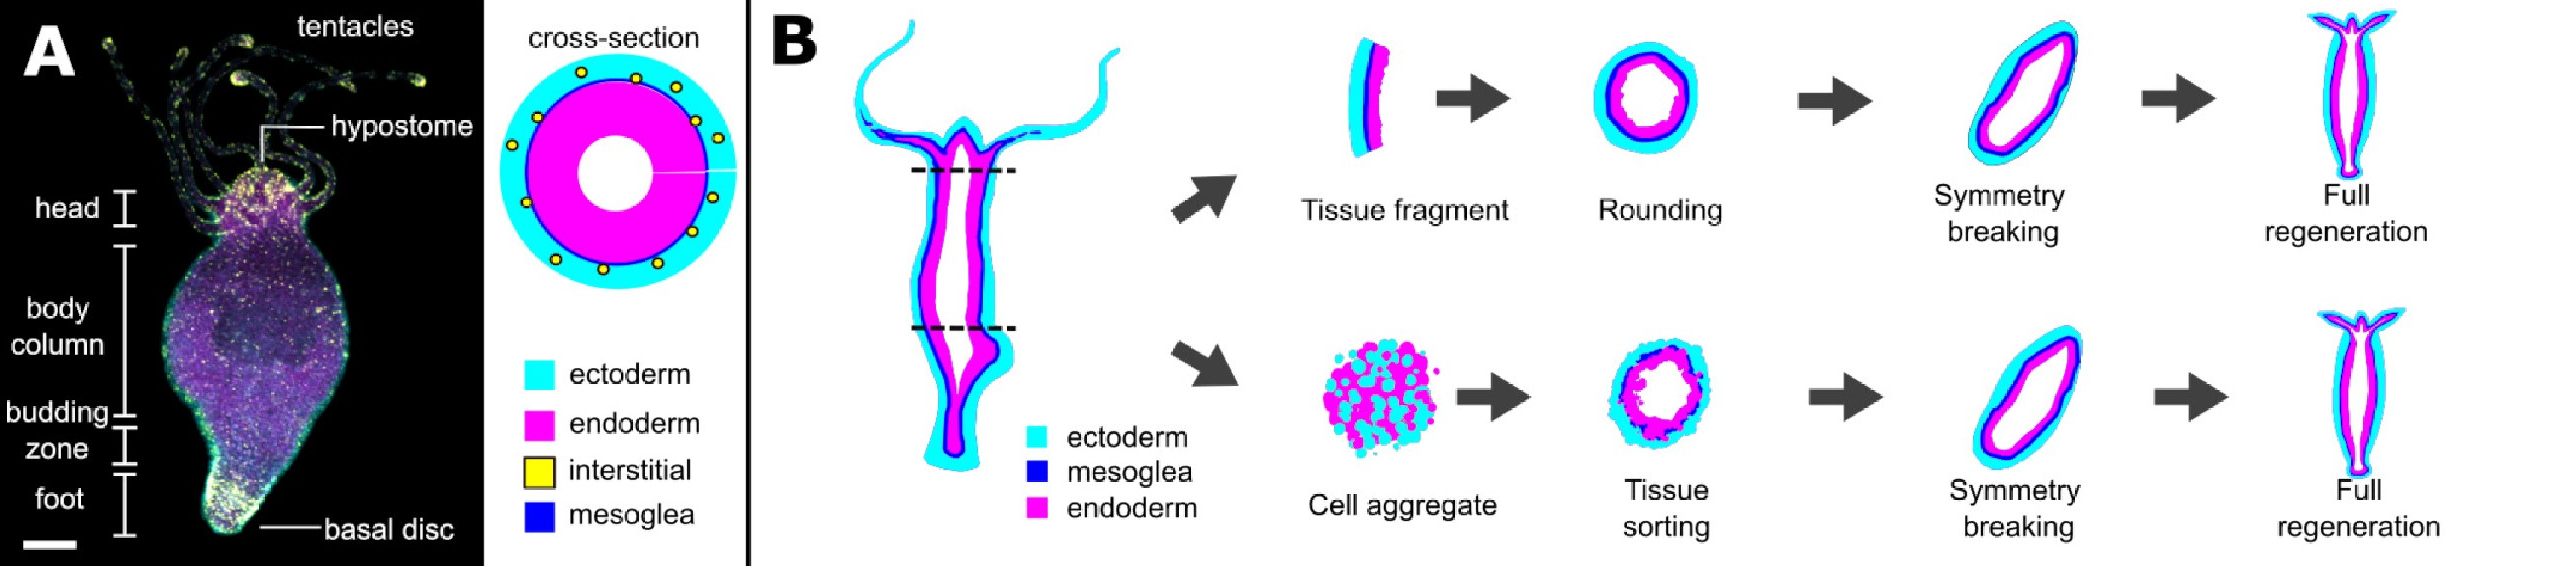
\includegraphics[
        width=\linewidth,
        height=5.20cm,
        keepaspectratio
      ]{figures/mechanochemistry/hydra_biology.png}
    \end{column}

    \begin{column}{0.29\textwidth}
      \HydraPoint[HydraGold]
        {Initially symmetric}
        {A tissue fragment rounds into a hollow spheroid}
      \vspace{-0.08cm}
      \HydraPoint[HydraCyan]
        {Symmetry is broken}
        {One region becomes the future head organizer}
      \vspace{-0.08cm}
      \HydraPoint[HydraGreen]
        {A complete axis emerges}
        {The localized organizer directs whole-body regeneration}
    \end{column}
  \end{columns}

  \source{Wang et al., Integrative and Comparative Biology, 2023}

\end{frame}


\begin{frame}{The central question}

  \vspace{0.40cm}

  \begin{center}
    \begin{minipage}{0.84\linewidth}
      \centering
      {\color{HydraMuted}\fontsize{8.2}{10}\selectfont
        Can a local morphogen change the mechanics of the entire spheroid?
      \par}
      \vspace{0.36cm}
      {\color{HydraWhite}\bfseries\fontsize{18}{23}\selectfont
        Can mechanics replace the diffusible inhibitor?
      \par}
      \vspace{0.46cm}
      {\color{HydraCyan}\fontsize{20}{20}\selectfont $\Downarrow$\par}
      \vspace{0.40cm}
      {\color{HydraGold}\bfseries\fontsize{12}{15}\selectfont
        Build the simplest mechanochemical model that can answer this question
      \par}
    \end{minipage}
  \end{center}

\end{frame}


\HydraSubsection[
  \mbox{Swelling and rupture expose}
  \mbox{a two-way coupling between}
  \mbox{morphogen signaling and mechanics}
]{Mechanics during regeneration}


\begin{frame}{One oscillation is a swelling and rupture cycle}

  \vspace{0.22cm}

  \HydraProcess{water enters}{tissue stretches}{tissue ruptures}

  \vspace{0.54cm}

  \begin{center}
    {\color{HydraCyan}\fontsize{19}{19}\selectfont $\Downarrow$}

    \vspace{0.28cm}

    {\color{HydraGreen}\bfseries\fontsize{12}{15}\selectfont
      the tissue deflates, heals, and the cycle begins again
    \par}
  \end{center}

  \vspace{0.46cm}

  \HydraTakeaway{
    Osmotic pressure repeatedly converts fluid transport into tissue stretching
  }

\end{frame}


\begin{frame}{The spheroid radius records repeated rupture events}

  \vspace{-0.18cm}

  \begin{columns}[c,onlytextwidth]
    \begin{column}{0.72\textwidth}
      \centering
      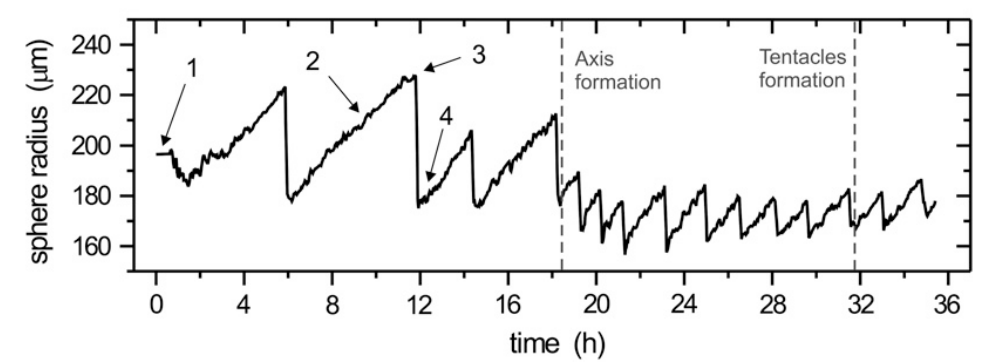
\includegraphics[
        width=\linewidth,
        height=5.25cm,
        keepaspectratio
      ]{figures/mechanochemistry/oscillation_radius.png}
    \end{column}

    \begin{column}{0.24\textwidth}
      \HydraPoint[HydraGold]
        {Slow increase}
        {Water influx gradually increases the spheroid radius}
      \vspace{-0.06cm}
      \HydraPoint[HydraRed]
        {Rapid decrease}
        {Rupture releases fluid and abruptly reduces the radius}
      \vspace{-0.06cm}
      \HydraPoint[HydraCyan]
        {Changing dynamics}
        {The oscillation changes as the body axis and tentacles form}
    \end{column}
  \end{columns}

  \source{Kuecken et al., Biophysical Journal, 2008}

\end{frame}


\begin{frame}{Wnt3 changes the oscillatory dynamics}

  \vspace{-0.18cm}

  \begin{columns}[c,onlytextwidth]
    \begin{column}{0.72\textwidth}
      \centering
      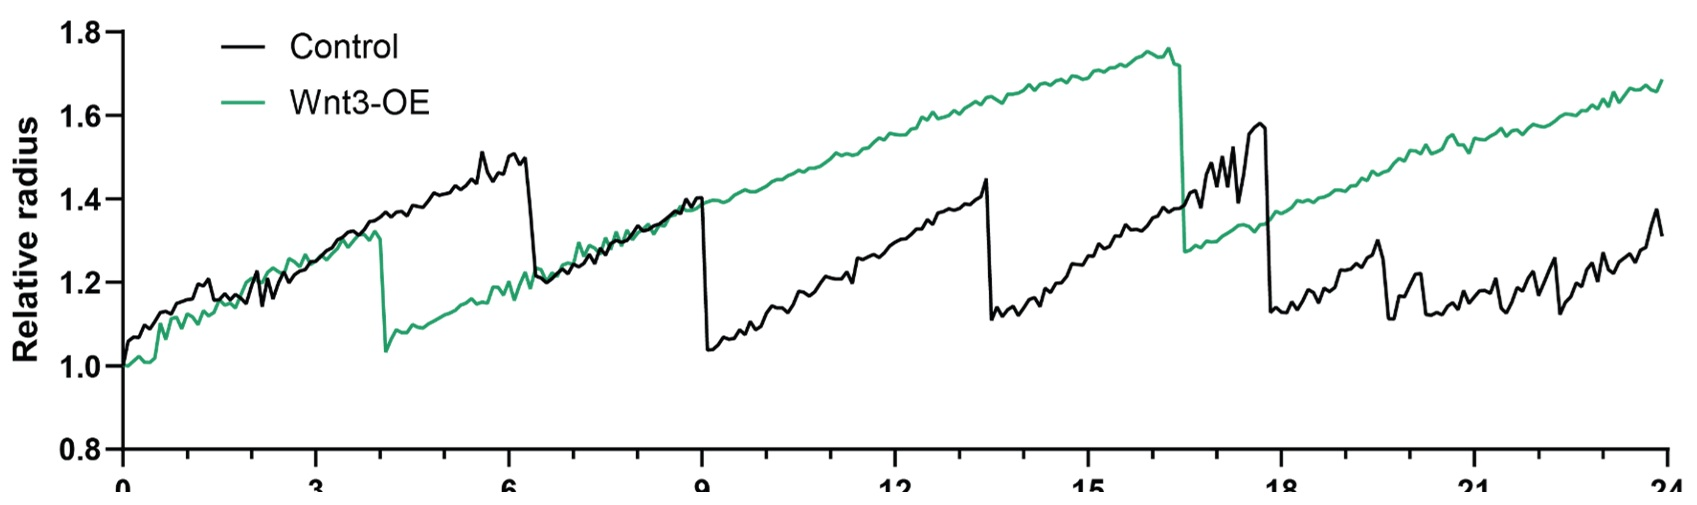
\includegraphics[
        width=\linewidth,
        height=5.15cm,
        keepaspectratio
      ]{figures/mechanochemistry/oscillation_wnt3_oe.jpg}
    \end{column}

    \begin{column}{0.24\textwidth}
      \HydraPoint[HydraGold]
        {Control}
        {Repeated rupture limits the gradual increase in radius}
      \vspace{-0.02cm}
      \HydraPoint[HydraGreen]
        {Wnt3 overexpression}
        {The timing and amplitude of rupture events are altered}
      \vspace{-0.02cm}
      {\color{HydraMuted}\fontsize{7.1}{8.7}\selectfont
        Morphogen signaling and tissue-scale mechanics cannot be treated independently
      \par}
    \end{column}
  \end{columns}

\end{frame}


\begin{frame}{Experiments suggest a mechanochemical coupling}

  \vspace{0.10cm}

  \begin{columns}[c,onlytextwidth]
    \begin{column}{0.44\textwidth}
      \centering
      {\color{HydraGold}\bfseries\fontsize{9.2}{11}\selectfont TISSUE STRETCHING\par}
      \vspace{0.32cm}
      {\color{HydraCyan}\fontsize{19}{19}\selectfont $\Downarrow$}
      \vspace{0.28cm}
      {\color{HydraWhite}\bfseries\fontsize{11.5}{14}\selectfont Wnt3 production\par}
      \vspace{0.24cm}
      {\color{HydraMuted}\fontsize{7.3}{9}\selectfont
        Stretching correlates with organizer formation and Wnt3 expression
      \par}
    \end{column}

    \begin{column}{0.08\textwidth}
      \centering{\color{HydraLine}\fontsize{30}{30}\selectfont $\vert$}
    \end{column}

    \begin{column}{0.44\textwidth}
      \centering
      {\color{HydraWhite}\bfseries\fontsize{11.5}{14}\selectfont MORPHOGEN\par}
      \vspace{0.32cm}
      {\color{HydraCyan}\fontsize{19}{19}\selectfont $\Downarrow$}
      \vspace{0.28cm}
      {\color{HydraGreen}\bfseries\fontsize{10.2}{12.5}\selectfont Tissue elasticity\par}
      \vspace{0.24cm}
      {\color{HydraMuted}\fontsize{7.3}{9}\selectfont
        Morphogen signaling changes how strongly the tissue resists deformation
      \par}
    \end{column}
  \end{columns}

  \vspace{0.52cm}
  \HydraTakeaway{Each side of the feedback modifies the other}

\end{frame}


\begin{frame}{Mechanochemical feedback}

  \vspace{-0.18cm}

  \begin{columns}[c,onlytextwidth]
    \begin{column}{0.62\textwidth}
      \centering
      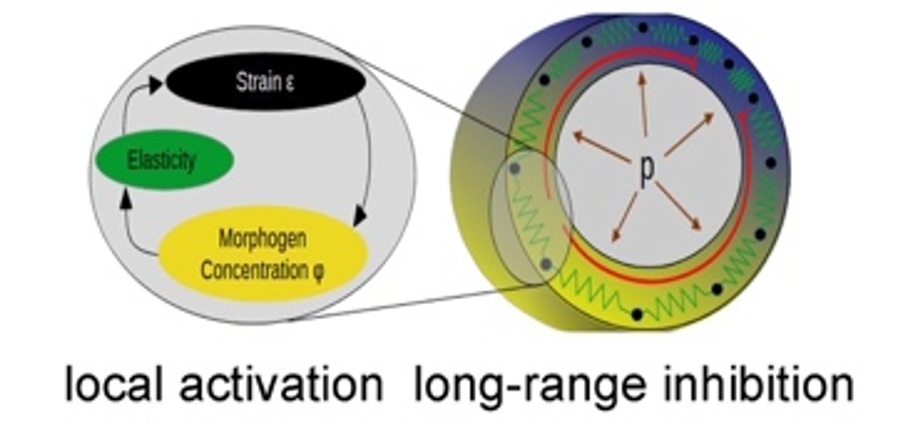
\includegraphics[
        width=\linewidth,
        height=5.35cm,
        keepaspectratio
      ]{figures/mechanochemistry/3d_intersection.jpg}
    \end{column}

    \begin{column}{0.34\textwidth}
      \HydraPoint[HydraGold]
        {Local activation}
        {Morphogen changes elasticity and concentrates strain locally}
      \vspace{-0.05cm}
      \HydraPoint[HydraCyan]
        {Long-range inhibition}
        {The closed pressurized tissue shares a finite total deformation}
      \vspace{-0.05cm}
      \HydraPoint[HydraGold]
        {Minimal ingredients}
        {Morphogen dynamics, mechanics and one global constraint}
    \end{column}
  \end{columns}

\end{frame}

\HydraSubsection[
  \mbox{A closed ring of springs reveals}
  \mbox{how local elasticity produces}
  \mbox{a global redistribution of strain}
]{From springs to a continuum}


% \begin{frame}{Replace the spheroid by an elastic ring}

%   \vspace{-0.18cm}

%   \begin{columns}[c,onlytextwidth]
%     \begin{column}{0.48\textwidth}
%       \centering
%       
\includegraphics[
%         width=\linewidth,
%         height=4.95cm,
%         keepaspectratio
%       ]{figures/mechanochemistry/sphere_springs.png}
%     \end{column}

%     \begin{column}{0.48\textwidth}
%       \HydraPoint[HydraGold]
%         {Closed geometry}
%         {The one-dimensional ring represents a cross-section of the spheroid}
%       \vspace{-0.04cm}
%       \HydraPoint[HydraCyan]
%         {Elastic tissue}
%         {Neighbouring material points are connected by springs}
%       \vspace{-0.04cm}
%       \HydraPoint[HydraGreen]
%         {Morphogen-dependent stiffness}
%         {Each spring responds to the local concentration of morphogen}
%     \end{column}
%   \end{columns}

%   \HydraTakeaway{
%     The ring retains the essential coupling while removing unnecessary geometry
%   }

% \end{frame}


\begin{frame}{Local changes redistribute strain around the ring}

  \vspace{-0.18cm}

  \begin{columns}[c,onlytextwidth]
    \begin{column}{0.65\textwidth}
      \centering
      \begin{tikzpicture}[x=1cm,y=1cm]
        \fill[HydraPanel] (0.20,0.25) rectangle (9.45,5.05);
        \draw[HydraLine,line width=1.0pt,rounded corners=3pt]
          (0.20,0.25) rectangle (9.45,5.05);
        \foreach \a in {0,30,...,330}{
          \fill[HydraWhite]
            ({4.82+1.72*cos(\a)},{2.65+1.72*sin(\a)}) circle[radius=0.055cm];
        }
        \draw[HydraCyan,line width=1.0pt]
          plot[domain=0:360,samples=13]
            ({4.82+1.72*cos(\x)},{2.65+1.72*sin(\x)});
        \fill[HydraGold] ({4.82+1.72*cos(30)},{2.65+1.72*sin(30)}) circle[radius=0.12cm];
      \end{tikzpicture}
    \end{column}

    \begin{column}{0.31\textwidth}
      \HydraPoint[HydraGold]
        {Move one node}
        {A local displacement changes several neighboring springs}
      \vspace{-0.04cm}
      \HydraPoint[HydraCyan]
        {Change one stiffness}
        {A softer spring takes a larger share of the deformation}
      \vspace{-0.04cm}
      \HydraPoint[HydraGold]
        {Close the ring}
        {The total extension cannot be assigned independently at every point}
    \end{column}
  \end{columns}

\end{frame}


\begin{frame}{A ring contains many small springs}

  \vspace{-0.14cm}

  \begin{columns}[c,onlytextwidth]
    \begin{column}{0.60\textwidth}
      \centering
      \begin{tikzpicture}[x=0.95cm,y=0.95cm]
        \def\R{2.45}
        \coordinate (O) at (3.40,2.75);
        \foreach \a in {0,20,...,340}{
          \fill[HydraWhite] ($(O)+(\a:\R)$) circle[radius=0.060cm];
        }
        \draw[HydraCyan,line width=1.0pt]
          plot[domain=0:360,samples=19]
            ({3.40+\R*cos(\x)},{2.75+\R*sin(\x)});
        \fill[HydraGold] ($(O)+(40:\R)$) circle[radius=0.105cm];
        \fill[HydraGold] ($(O)+(60:\R)$) circle[radius=0.105cm];
        \draw[HydraGold,line width=2.0pt]
          ($(O)+(40:\R)$) -- ($(O)+(60:\R)$);
        \node[anchor=south west,text=HydraGold,
          font=\bfseries\fontsize{7.4}{8.8}\selectfont]
          at ($(O)+(50:2.72)$) {spring $i$};
        \node[text=HydraMuted,font=\fontsize{7}{8.5}\selectfont]
          at (3.40,2.75) {$N$ springs};
      \end{tikzpicture}
    \end{column}

    \begin{column}{0.36\textwidth}
      {\color{HydraWhite}\fontsize{10}{12.6}\selectfont
      \begin{align*}
        \Delta x&=\frac{L}{N}
        \\
        x_i&=i\Delta x
        \\
        i&=0,\ldots,N-1
      \end{align*}
      }
      \par
      \vspace{-0.32cm}
      {\color{HydraMuted}\fontsize{7.5}{9.2}\selectfont
        Every spring represents a short material segment of reference length $\Delta x$
      \par}
    \end{column}
  \end{columns}

\end{frame}


\begin{frame}{Compare the reference and deformed spring}

  \vspace{0.05cm}

  \begin{columns}[c,onlytextwidth]
    \begin{column}{0.46\textwidth}
      \centering
      {\color{HydraGold}\bfseries\fontsize{8}{9.5}\selectfont
        REFERENCE CONFIGURATION\par}
      \vspace{0.30cm}
      \begin{tikzpicture}[x=1cm,y=1cm]
        \fill[HydraWhite] (0.55,2.10) circle[radius=0.095cm];
        \fill[HydraWhite] (5.10,2.10) circle[radius=0.095cm];
        \draw[HydraLine,line width=1.6pt] (0.55,2.10) -- (5.10,2.10);
        \draw[<->,HydraGold,line width=1.0pt] (0.55,1.35) -- (5.10,1.35);
        \node[text=HydraGold,font=\bfseries\fontsize{8}{9.5}\selectfont]
          at (2.82,0.92) {$\Delta x$};
      \end{tikzpicture}
    \end{column}

    \begin{column}{0.06\textwidth}
      \centering{\color{HydraCyan}\fontsize{19}{19}\selectfont $\Rightarrow$}
    \end{column}

    \begin{column}{0.46\textwidth}
      \centering
      {\color{HydraCyan}\bfseries\fontsize{8}{9.5}\selectfont
        DEFORMED CONFIGURATION\par}
      \vspace{0.30cm}
      \begin{tikzpicture}[x=1cm,y=1cm]
        \fill[HydraWhite] (0.30,2.10) circle[radius=0.095cm];
        \fill[HydraWhite] (5.55,2.10) circle[radius=0.095cm];
        \draw[HydraCyan,line width=1.6pt] (0.30,2.10) -- (5.55,2.10);
        \draw[<->,HydraCyan,line width=1.0pt] (0.30,1.35) -- (5.55,1.35);
        \node[text=HydraCyan,font=\bfseries\fontsize{8}{9.5}\selectfont]
          at (2.92,0.92) {$\ell_i$};
      \end{tikzpicture}
    \end{column}
  \end{columns}

  \vspace{0.38cm}

  {\color{HydraWhite}\fontsize{10.5}{13.2}\selectfont
  \begin{align*}
    \text{extension of spring } i
    &: \quad \ell_i-\Delta x
  \end{align*}
  }

\end{frame}


\begin{frame}{Strain measures relative extension}

  \vspace{0.18cm}

  \begin{center}
    \begin{minipage}{0.78\linewidth}
      {\color{HydraMuted}\fontsize{8}{9.8}\selectfont
        Absolute extension depends on the size of the spring
      \par}
      \vspace{-0.16cm}
      {\color{HydraWhite}\bfseries\fontsize{15}{18.5}\selectfont
      \begin{align*}
        \boxed{
          \varepsilon_i
          =
          \frac{\ell_i-\Delta x}{\Delta x}
        }
      \end{align*}
      }
      \par
      \vspace{-0.24cm}
      \HydraPoint[HydraCyan]
        {$\varepsilon_i=0$}
        {The spring keeps its reference length}
      \vspace{-0.12cm}
      \HydraPoint[HydraGold]
        {$\varepsilon_i>0$}
        {The spring is stretched}
      \vspace{-0.12cm}
      \HydraPoint[HydraGold]
        {$\varepsilon_i<0$}
        {The spring is compressed}
    \end{minipage}
  \end{center}

\end{frame}


\begin{frame}{The energy of one spring has the correct continuum scaling}

  \vspace{-0.10cm}

  \begin{columns}[c,onlytextwidth]
    \begin{column}{0.52\textwidth}
      {\color{HydraMuted}\fontsize{7.8}{9.5}\selectfont
        Hooke's law assigns the spring energy
      \par}
      \vspace{-0.18cm}
      {\color{HydraWhite}\fontsize{10.2}{12.9}\selectfont
      \begin{align*}
        \mathcal E_i
        &=
        \frac12k_i(u_i)
        \left(\ell_i-\Delta x\right)^2
        \\
        k_i(u_i)&=\frac{E(u_i)}{\Delta x}
      \end{align*}
      }
      \par
      \vspace{-0.34cm}
      {\color{HydraGold}\bfseries\fontsize{11.2}{14.2}\selectfont
      \begin{align*}
        \boxed{
          \mathcal E_i
          =
          \frac12E(u_i)\varepsilon_i^2\Delta x
        }
      \end{align*}
      }
    \end{column}

    \begin{column}{0.44\textwidth}
      \HydraPoint[HydraGold]
        {Quadratic response}
        {Doubling the extension multiplies the elastic energy by four}
      \vspace{-0.04cm}
      \HydraPoint[HydraCyan]
        {Consistent subdivision}
        {Increasing the number of springs does not change the tissue stiffness}
      \vspace{-0.04cm}
      {\color{HydraMuted}\fontsize{7.2}{8.8}\selectfont
        The factor $\Delta x$ prepares the energy for a Riemann-sum limit
      \par}
    \end{column}
  \end{columns}

\end{frame}


\begin{frame}{Morphogen concentration controls local stiffness}

  \vspace{-0.06cm}

  \begin{columns}[c,onlytextwidth]
    \begin{column}{0.48\textwidth}
      {\color{HydraWhite}\bfseries\fontsize{12.2}{15.4}\selectfont
      \begin{align*}
        E'(u)&<0
      \end{align*}
      }
      \par
      \vspace{-0.26cm}
      \HydraPoint[HydraGold]
        {High morphogen}
        {The elastic modulus is smaller and the tissue is softer}
      \vspace{-0.06cm}
      \HydraPoint[HydraCyan]
        {Low morphogen}
        {The elastic modulus is larger and the tissue is stiffer}
      \vspace{-0.12cm}
      {\color{HydraWhite}\fontsize{10.3}{13}\selectfont
      \begin{align*}
        E(u)&=e^{-\beta u}
        \qquad
        \beta>0
      \end{align*}
      }
    \end{column}

    \begin{column}{0.48\textwidth}
      \centering
      \begin{tikzpicture}[x=0.92cm,y=0.92cm]
        \draw[-{Latex[length=2mm]},HydraMuted,line width=0.7pt]
          (0.45,0.55) -- (5.45,0.55)
          node[below,text=HydraMuted,font=\fontsize{7}{8.2}\selectfont] {$u$};
        \draw[-{Latex[length=2mm]},HydraMuted,line width=0.7pt]
          (0.55,0.45) -- (0.55,5.15)
          node[left,text=HydraMuted,font=\fontsize{7}{8.2}\selectfont] {$E(u)$};
        \draw[HydraGold,line width=1.7pt,domain=0.55:5.10,samples=100]
          plot (\x,{0.60+4.05*exp(-0.58*(\x-0.55))});
        \node[anchor=west,text=HydraGold,
          font=\bfseries\fontsize{7.4}{8.8}\selectfont]
          at (3.25,1.45) {$e^{-\beta u}$};
      \end{tikzpicture}
    \end{column}
  \end{columns}

\end{frame}


\begin{frame}{The local feedback is positive}

  \vspace{0.35cm}

  \begin{columns}[c,onlytextwidth]
    \begin{column}{0.24\textwidth}
      \centering{\color{HydraGold}\bfseries\fontsize{10}{12}\selectfont higher $u$\par}
    \end{column}
    \begin{column}{0.06\textwidth}
      \centering{\color{HydraCyan}\fontsize{17}{17}\selectfont $\Rightarrow$}
    \end{column}
    \begin{column}{0.24\textwidth}
      \centering{\color{HydraWhite}\bfseries\fontsize{10}{12}\selectfont smaller $E(u)$\par}
    \end{column}
    \begin{column}{0.06\textwidth}
      \centering{\color{HydraCyan}\fontsize{17}{17}\selectfont $\Rightarrow$}
    \end{column}
    \begin{column}{0.18\textwidth}
      \centering{\color{HydraCyan}\bfseries\fontsize{10}{12}\selectfont larger strain\par}
    \end{column}
    \begin{column}{0.06\textwidth}
      \centering{\color{HydraCyan}\fontsize{17}{17}\selectfont $\Rightarrow$}
    \end{column}
    \begin{column}{0.16\textwidth}
      \centering{\color{HydraGreen}\bfseries\fontsize{10}{12}\selectfont more $u$\par}
    \end{column}
  \end{columns}

  \vspace{0.70cm}

  \begin{center}
    \begin{minipage}{0.78\linewidth}
      \HydraPoint[HydraGold]
        {Local activation}
        {A small local increase in morphogen makes the same region easier to stretch}
      \vspace{-0.10cm}
      \HydraPoint[HydraCyan]
        {Missing ingredient}
        {We still need to determine how the strain is distributed around the entire ring}
    \end{minipage}
  \end{center}

\end{frame}


\begin{frame}{The total discrete energy is a sum over all springs}

  \vspace{0.10cm}

  \begin{center}
    \begin{minipage}{0.82\linewidth}
      {\color{HydraMuted}\fontsize{8}{9.8}\selectfont
        Every spring contributes its local elastic energy
      \par}
      \vspace{-0.10cm}
      {\color{HydraWhite}\bfseries\fontsize{14.2}{17.8}\selectfont
      \begin{align*}
        \mathcal E_N
        =
        \sum_{i=0}^{N-1}\mathcal E_i=
        \sum_{i=0}^{N-1}
        \frac12E(u_i)\varepsilon_i^2\Delta x
      \end{align*}
      }
      \par
      \vspace{-0.28cm}
      \HydraPoint[HydraGold]
        {Local contribution}
        {Each term depends only on the strain and morphogen at spring $i$}
      \vspace{-0.10cm}
      \HydraPoint[HydraCyan]
        {Global configuration}
        {The total energy depends on how deformation is shared by all springs}
    \end{minipage}
  \end{center}

\end{frame}


\begin{frame}{A material coordinate follows the tissue}

  \vspace{-0.06cm}

  \begin{columns}[c,onlytextwidth]
    \begin{column}{0.58\textwidth}
      \centering
      \begin{tikzpicture}[x=0.96cm,y=0.96cm]
        \draw[HydraLine,line width=1.2pt] (2.05,2.75) circle[radius=1.45cm];
        \draw[HydraCyan,line width=1.2pt] (6.25,2.75) circle[radius=2.05cm];
        \fill[HydraGold] ({2.05+1.45*cos(35)},{2.75+1.45*sin(35)}) circle[radius=0.09cm];
        \fill[HydraGold] ({6.25+2.05*cos(35)},{2.75+2.05*sin(35)}) circle[radius=0.09cm];
        \draw[-{Latex[length=2.5mm]},HydraGold,line width=1.0pt]
          ({2.05+1.55*cos(35)},{2.75+1.55*sin(35)}) .. controls (4.00,4.80) ..
          ({6.25+1.95*cos(35)},{2.75+1.95*sin(35)});
        \node[text=HydraMuted,font=\fontsize{7.2}{8.7}\selectfont]
          at (2.05,0.78) {reference ring $[0,L]$};
        \node[text=HydraCyan,font=\fontsize{7.2}{8.7}\selectfont]
          at (6.25,0.20) {deformed ring $[0,\ell]$};
        \node[text=HydraGold,font=\bfseries\fontsize{7.2}{8.7}\selectfont]
          at (4.20,4.88) {$s(x)$};
      \end{tikzpicture}
    \end{column}

    \begin{column}{0.38\textwidth}
      {\color{HydraWhite}\fontsize{10.6}{13.4}\selectfont
      \begin{align*}
        x&\in[0,L]
        \\
        s(x)&\in[0,\ell]
      \end{align*}
      }
      \par
      \vspace{-0.25cm}
      \HydraPoint[HydraGold]
        {Material label}
        {$x$ identifies a fixed piece of tissue}
      \vspace{-0.06cm}
      \HydraPoint[HydraCyan]
        {Deformed position}
        {$s(x)$ gives its arc-length position after stretching}
    \end{column}
  \end{columns}

\end{frame}


\begin{frame}{Discrete strain converges to a spatial derivative}

  \vspace{0.05cm}

  \begin{center}
    \begin{minipage}{0.86\linewidth}
      {\color{HydraWhite}\fontsize{10.6}{13.4}\selectfont
      \begin{align*}
        \ell_i
        &=s(x_{i+1})-s(x_i)
        \\
        \varepsilon_i
        &=
        \frac{s(x_{i+1})-s(x_i)}{\Delta x}-1
      \end{align*}
      }
      \par
      \vspace{-0.28cm}
      \begin{center}
        {\color{HydraCyan}\fontsize{17}{17}\selectfont
          $\Delta x\longrightarrow0$
          \qquad
          $\Rightarrow$
        }
      \end{center}
      \vspace{-0.04cm}
      {\color{HydraWhite}\bfseries\fontsize{14.5}{18}\selectfont
      \begin{align*}
        \boxed{\varepsilon(x)=\partial_xs(x)-1}
      \end{align*}
      }
      \par
      \vspace{-0.24cm}
      {\color{HydraMuted}\fontsize{7.6}{9.3}\selectfont
        The strain compares the local deformed length with the reference length
      \par}
    \end{minipage}
  \end{center}

\end{frame}


\begin{frame}{The spring sum becomes a continuum energy}

  \vspace{0.14cm}

  \begin{center}
    \begin{minipage}{0.90\linewidth}
      {\color{HydraWhite}\fontsize{11}{13.8}\selectfont
      \begin{align*}
        \mathcal E_N
        &=
        \sum_{i=0}^{N-1}
        \frac12E(u_i)\varepsilon_i^2\Delta x
      \end{align*}
      }
      \par
      \vspace{-0.24cm}
      \begin{center}
        {\color{HydraCyan}\fontsize{18}{18}\selectfont
          $N\longrightarrow\infty$
          \qquad
          $\Downarrow$
        }
      \end{center}
      \vspace{-0.04cm}
      {\color{HydraGold}\bfseries\fontsize{15}{18.5}\selectfont
      \begin{align*}
        \boxed{
          \mathcal E_{\mathrm{el}}[s;u]
          =
          \frac12\int_0^L E(u(x))\varepsilon(x)^2\,dx
        }
      \end{align*}
      }
      \par
      \vspace{-0.22cm}
      {\color{HydraMuted}\fontsize{7.6}{9.3}\selectfont
        The discrete spring model has become a continuum elastic energy
      \par}
    \end{minipage}
  \end{center}

\end{frame}


\begin{frame}{The closed ring imposes a global length constraint}

  \vspace{0.04cm}

  \begin{columns}[c,onlytextwidth]
    \begin{column}{0.53\textwidth}
      {\color{HydraWhite}\fontsize{10.8}{13.6}\selectfont
      \begin{align*}
        \ell-L
        &=
        \sum_{i=0}^{N-1}
        \left(\ell_i-\Delta x\right)
        \\
        &=
        \sum_{i=0}^{N-1}\varepsilon_i\Delta x
      \end{align*}
      }
      \par
      \vspace{-0.26cm}
      \begin{center}{\color{HydraCyan}\fontsize{17}{17}\selectfont $\Downarrow$}\end{center}
      \vspace{-0.08cm}
      {\color{HydraGold}\bfseries\fontsize{13.2}{16.5}\selectfont
      \begin{align*}
        \boxed{\ell-L=\int_0^L\varepsilon(x)\,dx}
      \end{align*}
      }
    \end{column}

    \begin{column}{0.43\textwidth}
      \HydraPoint[HydraGold]
        {Total extension is prescribed}
        {Inflation determines how much longer the deformed ring is}
      \vspace{-0.02cm}
      \HydraPoint[HydraCyan]
        {Local strains are coupled}
        {More extension in one region leaves less extension for the rest of the ring}
    \end{column}
  \end{columns}

\end{frame}


\begin{frame}{Mechanical equilibrium minimizes elastic energy}

  \vspace{0.10cm}

  \begin{center}
    \begin{minipage}{0.84\linewidth}
      {\color{HydraMuted}\fontsize{7.8}{9.5}\selectfont
        Mechanics relaxes rapidly compared with morphogen dynamics
      \par}
      \vspace{-0.10cm}
      {\color{HydraWhite}\bfseries\fontsize{13.2}{16.6}\selectfont
      \begin{align*}
        s
        &\in
        \operatorname*{arg\,min}
        \left\{
          \frac12\int_0^L E(u)\varepsilon^2\,dx
        \right\}
      \end{align*}
      }
      \par
      \vspace{-0.26cm}
      {\color{HydraWhite}\fontsize{10.4}{13.2}\selectfont
      \begin{align*}
        \varepsilon&=\partial_xs-1
        \\
        \int_0^L\varepsilon\,dx&=\ell-L
      \end{align*}
      }
      \par
      \vspace{-0.28cm}
      \HydraPoint[HydraGold]
        {Quasi-static mechanics}
        {For each current morphogen profile the tissue immediately reaches mechanical equilibrium}
    \end{minipage}
  \end{center}

\end{frame}


\begin{frame}{Perturb the deformation to compute the first variation}

  \vspace{0.02cm}

  \begin{columns}[c,onlytextwidth]
    \begin{column}{0.47\textwidth}
      {\color{HydraWhite}\fontsize{10.4}{13.2}\selectfont
      \begin{align*}
        s_\theta(x)&=s(x)+\theta h(x)
        \\
        \varepsilon_\theta&=\partial_xs_\theta-1
        \\
        &=\varepsilon+\theta\partial_xh
      \end{align*}
      }
      \par
      \vspace{-0.30cm}
      {\color{HydraMuted}\fontsize{7.4}{9.1}\selectfont
        The periodic perturbation $h$ preserves the closed geometry
      \par}
    \end{column}

    \begin{column}{0.49\textwidth}
      {\color{HydraWhite}\fontsize{9.6}{12.2}\selectfont
      \begin{align*}
        \mathcal E_{\mathrm{el}}[s_\theta;u]
        &=
        \frac12\int_0^L
        E(u)
        \left(\varepsilon+\theta\partial_xh\right)^2\,dx
      \end{align*}
      }
      \par
      \vspace{-0.26cm}
      {\color{HydraGold}\bfseries\fontsize{10.5}{13.2}\selectfont
      \begin{align*}
        \delta\mathcal E_{\mathrm{el}}
        &=
        \left.\frac{d}{d\theta}
        \mathcal E_{\mathrm{el}}[s_\theta;u]
        \right|_{\theta=0}
        \\
        &=\int_0^L E(u)\varepsilon\partial_xh\,dx
      \end{align*}
      }
    \end{column}
  \end{columns}

\end{frame}


\begin{frame}{Integration by parts gives mechanical equilibrium}

  \vspace{0.12cm}

  \begin{center}
    \begin{minipage}{0.88\linewidth}
      {\color{HydraWhite}\fontsize{10.5}{13.2}\selectfont
      \begin{align*}
        \delta\mathcal E_{\mathrm{el}}
        &=\int_0^L E(u)\varepsilon\partial_xh\,dx
        \\
        &=-\int_0^L
        \partial_x\!\left(E(u)\varepsilon\right)h\,dx
      \end{align*}
      }
      \par
      \vspace{-0.24cm}
      {\color{HydraMuted}\fontsize{7.7}{9.4}\selectfont
        The first variation vanishes for every admissible perturbation $h$
      \par}
      \vspace{-0.14cm}
      {\color{HydraGold}\bfseries\fontsize{15}{18.5}\selectfont
      \begin{align*}
        \boxed{\partial_x\!\left(E(u)\varepsilon\right)=0}
      \end{align*}
      }
    \end{minipage}
  \end{center}

\end{frame}


\begin{frame}{Mechanical equilibrium determines the strain explicitly}

  \vspace{-0.14cm}

  {\color{HydraWhite}\fontsize{9.8}{12.5}\selectfont
  \begin{align*}
    E(u(x,t))\varepsilon(x,t)&=\sigma(t)
    \\
    \varepsilon(x,t)&=\frac{\sigma(t)}{E(u(x,t))}
  \end{align*}
  }
  \par
  \vspace{-0.38cm}
  {\color{HydraWhite}\fontsize{9.4}{12}\selectfont
  \begin{align*}
    \ell-L
    &=\sigma(t)\int_0^L\frac{1}{E(u(y,t))}\,dy
  \end{align*}
  }
  \par
  \vspace{-0.32cm}
  {\color{HydraGold}\bfseries\fontsize{11.5}{14.5}\selectfont
  \begin{align*}
    \boxed{
      \varepsilon(x,t)
      =
      \frac{\ell-L}
      {E(u(x,t))
      \displaystyle\int_0^L\frac{1}{E(u(y,t))}\,dy}
    }
  \end{align*}
  }

\end{frame}


\begin{frame}{The full model couples dynamics and mechanical equilibrium}

  \vspace{-0.12cm}

  \begin{columns}[c,onlytextwidth]
    \begin{column}{0.62\textwidth}
      {\color{HydraWhite}\fontsize{10.6}{13.4}\selectfont
      \begin{align*}
        \partial_tu
        &=D\partial_{xx}u-\alpha u+\kappa\varepsilon
        \\
        0
        &=\partial_x\!\left(E(u)\varepsilon\right)
        \\
        \ell-L
        &=\int_0^L\varepsilon(x,t)\,dx
      \end{align*}
      }
      \par
      \vspace{-0.24cm}
      {\color{HydraMuted}\fontsize{7.5}{9.2}\selectfont
        supplemented with periodic boundary conditions and an initial morphogen profile
      \par}
    \end{column}

    \begin{column}{0.34\textwidth}
      \HydraPoint[HydraGold]
        {One evolution equation}
        {Only the morphogen has its own time dynamics}
      \vspace{-0.04cm}
      \HydraPoint[HydraCyan]
        {Instantaneous mechanics}
        {Strain is determined by equilibrium at every time}
      \vspace{-0.04cm}
      \HydraPoint[HydraGold]
        {One global constraint}
        {The prescribed total extension couples the entire ring}
    \end{column}
  \end{columns}

\end{frame}


\begin{frame}{Mechanical variables can be eliminated exactly}

  \vspace{-0.12cm}

  {\color{HydraWhite}\fontsize{9.0}{11.4}\selectfont
  \begin{align*}
    \partial_tu
    &=D\partial_{xx}u-\alpha u+\kappa\varepsilon
    \\
    \varepsilon(x,t)
    &=
    \frac{\ell-L}
    {E(u(x,t))
    \displaystyle\int_0^L\frac{1}{E(u(y,t))}\,dy}
  \end{align*}
  }
  \par
  \vspace{-0.28cm}
  \begin{center}{\color{HydraCyan}\fontsize{17}{17}\selectfont $\Downarrow$}\end{center}
  \vspace{-0.08cm}
  {\color{HydraGold}\bfseries\fontsize{9.6}{12.2}\selectfont
  \begin{align*}
    \boxed{
      \partial_tu
      =D\partial_{xx}u-\alpha u
      +\kappa
      \frac{\ell-L}
      {E(u(x,t))
      \displaystyle\int_0^L\frac{1}{E(u(y,t))}\,dy}
    }
  \end{align*}
  }

\end{frame}


\begin{frame}{Exponential softening produces the nonlocal feedback}

  \vspace{-0.02cm}

  \begin{columns}[c,onlytextwidth]
    \begin{column}{0.43\textwidth}
      {\color{HydraWhite}\fontsize{10.6}{13.4}\selectfont
      \begin{align*}
        E(u)&=e^{-\beta u}
        \\
        \frac{1}{E(u)}&=e^{\beta u}
      \end{align*}
      }
      \par
      \vspace{-0.30cm}
      \HydraPoint[HydraGold]
        {Local factor}
        {$e^{\beta u(x,t)}$ amplifies regions with larger morphogen}
    \end{column}

    \begin{column}{0.53\textwidth}
      {\color{HydraGold}\bfseries\fontsize{10.8}{13.6}\selectfont
      \begin{align*}
        \varepsilon(x,t)
        &=
        (\ell-L)
        \frac{e^{\beta u(x,t)}}
        {\displaystyle\int_0^L e^{\beta u(y,t)}\,dy}
      \end{align*}
      }
      \par
      \vspace{-0.24cm}
      \HydraPoint[HydraCyan]
        {Global factor}
        {The denominator preserves the prescribed total extension}
    \end{column}
  \end{columns}

  \vspace{0.30cm}
  \HydraTakeaway{
    The mechanics generates a local exponential activation divided by a global normalization
  }

\end{frame}


\begin{frame}{Nondimensionalization gives one nonlocal equation}

  \vspace{-0.16cm}

  \begin{columns}[c,onlytextwidth]
    \begin{column}{0.35\textwidth}
      {\color{HydraMuted}\fontsize{7.4}{9.1}\selectfont
        Natural variables
      \par}
      \vspace{-0.22cm}
      {\color{HydraWhite}\fontsize{8.8}{11.2}\selectfont
      \begin{align*}
        \widetilde x&=\frac{x}{L}
        \\
        \widetilde t&=\alpha t
        \\
        \widetilde u&=\beta u
      \end{align*}
      }
    \end{column}

    \begin{column}{0.61\textwidth}
      {\color{HydraGold}\bfseries\fontsize{11.4}{14.4}\selectfont
      \begin{align*}
        \boxed{
          \partial_tu
          =D\partial_{xx}u-u
          +\kappa
          \frac{e^{u(x,t)}}
          {\displaystyle\int_0^1e^{u(y,t)}\,dy}
        }
      \end{align*}
      }
      \par
      \vspace{-0.26cm}
      {\color{HydraMuted}\fontsize{7.4}{9.1}\selectfont
        The tildes are dropped and the domain is the unit circle $\mathbb{T}=[0,1]$
      \par}
    \end{column}
  \end{columns}

  \vspace{0.30cm}

  {\color{HydraWhite}\fontsize{8.8}{11.2}\selectfont
  \begin{align*}
    u(0,t)&=u(1,t)
    &
    \partial_xu(0,t)&=\partial_xu(1,t)
    &
    u(x,0)&=u_0(x)
  \end{align*}
  }

\end{frame}


\begin{frame}{One equation realizes the activator--inhibitor paradigm}

  \vspace{-0.05cm}

  \begin{columns}[c,onlytextwidth]
    \begin{column}{0.46\textwidth}
      \centering
      {\color{HydraGold}\bfseries\fontsize{8.2}{9.8}\selectfont
        LOCAL ACTIVATION\par}
      \vspace{-0.18cm}
      {\color{HydraWhite}\fontsize{12.2}{15.3}\selectfont
      \begin{align*}
        e^{u(x,t)}
      \end{align*}
      }
      \par
      \vspace{-0.26cm}
      {\color{HydraMuted}\fontsize{7.5}{9.2}\selectfont
        A region with more morphogen becomes softer and receives more strain-driven production
      \par}
    \end{column}

    \begin{column}{0.08\textwidth}
      \centering{\color{HydraLine}\rule{0.6pt}{2.6cm}}
    \end{column}

    \begin{column}{0.46\textwidth}
      \centering
      {\color{HydraCyan}\bfseries\fontsize{8.2}{9.8}\selectfont
        LONG-RANGE INHIBITION\par}
      \vspace{-0.18cm}
      {\color{HydraWhite}\fontsize{12.2}{15.3}\selectfont
      \begin{align*}
        \int_0^1e^{u(y,t)}\,dy
      \end{align*}
      }
      \par
      \vspace{-0.26cm}
      {\color{HydraMuted}\fontsize{7.5}{9.2}\selectfont
        Increased production in one region reduces the share of extension available elsewhere
      \par}
    \end{column}
  \end{columns}

  \vspace{0.54cm}
  \HydraTakeaway{
    Mechanical equilibrium converts a local positive feedback into global competition
  }

\end{frame}


\HydraSubsection[
  \mbox{Variational structure determines}
  \mbox{when patterns exist and which}
  \mbox{stationary profiles can be stable}
]{Steady states and stability}


\begin{frame}{Stationary patterns solve a nonlocal boundary-value problem}

  \vspace{0.02cm}

  \begin{columns}[c,onlytextwidth]
    \begin{column}{0.62\textwidth}
      {\color{HydraWhite}\fontsize{11}{13.9}\selectfont
      \begin{align*}
        0
        &=D\partial_{xx}U-U
        +\kappa
        \frac{e^{U(x)}}
        {\displaystyle\int_0^1e^{U(y)}\,dy}
      \end{align*}
      }
      \par
      \vspace{-0.20cm}
      {\color{HydraWhite}\fontsize{9.8}{12.5}\selectfont
      \begin{align*}
        U(0)&=U(1)
        \\
        \partial_xU(0)&=\partial_xU(1)
      \end{align*}
      }
    \end{column}

    \begin{column}{0.34\textwidth}
      \HydraPoint[HydraGold]
        {Homogeneous solution}
        {$\bar U\equiv\kappa$ is always a stationary solution}
      \vspace{-0.04cm}
      \HydraPoint[HydraCyan]
        {Patterned solution}
        {A nonconstant periodic function $U(x)$ represents a spatial pattern}
    \end{column}
  \end{columns}

  \vspace{0.18cm}

  {\color{HydraMuted}\fontsize{7.4}{9.1}\selectfont
    Every stationary solution has mean value $\int_0^1U(x)\,dx=\kappa$
  \par}

\end{frame}


\begin{frame}{Small diffusion permits patterns while large diffusion suppresses them}

  \vspace{-0.16cm}

  {\color{HydraGold}\bfseries\fontsize{8.2}{9.8}\selectfont
    THEOREM\par}

  \vspace{0.12cm}

  {\color{HydraWhite}\fontsize{8.5}{10.7}\selectfont
    For every $\kappa>0$ there exist constants
  \par}

  \vspace{-0.34cm}

  {\color{HydraWhite}\bfseries\fontsize{11.2}{14.2}\selectfont
  \begin{align*}
    0<D_{\min}(\kappa)<D_{\max}(\kappa)
  \end{align*}
  }

  \vspace{-0.36cm}

  \begin{columns}[T,onlytextwidth]
    \begin{column}{0.48\textwidth}
      \HydraPoint[HydraGold]
        {$0<D<D_{\min}(\kappa)$}
        {A nonconstant stationary solution exists and is Lyapunov stable in $L^2$}
    \end{column}

    \begin{column}{0.48\textwidth}
      \HydraPoint[HydraCyan]
        {$D>D_{\max}(\kappa)$}
        {$\bar U\equiv\kappa$ is the unique stationary solution and is globally asymptotically stable}
    \end{column}
  \end{columns}

  \vspace{0.20cm}

  {\color{HydraMuted}\fontsize{7.4}{9.1}\selectfont
    The analytic thresholds are sufficient bounds and need not be optimal
  \par}

\end{frame}


\begin{frame}{The parameter plane separates homogeneous and patterned regimes}

  \vspace{-0.16cm}

  \begin{columns}[c,onlytextwidth]
    \begin{column}{0.74\textwidth}
      \centering
      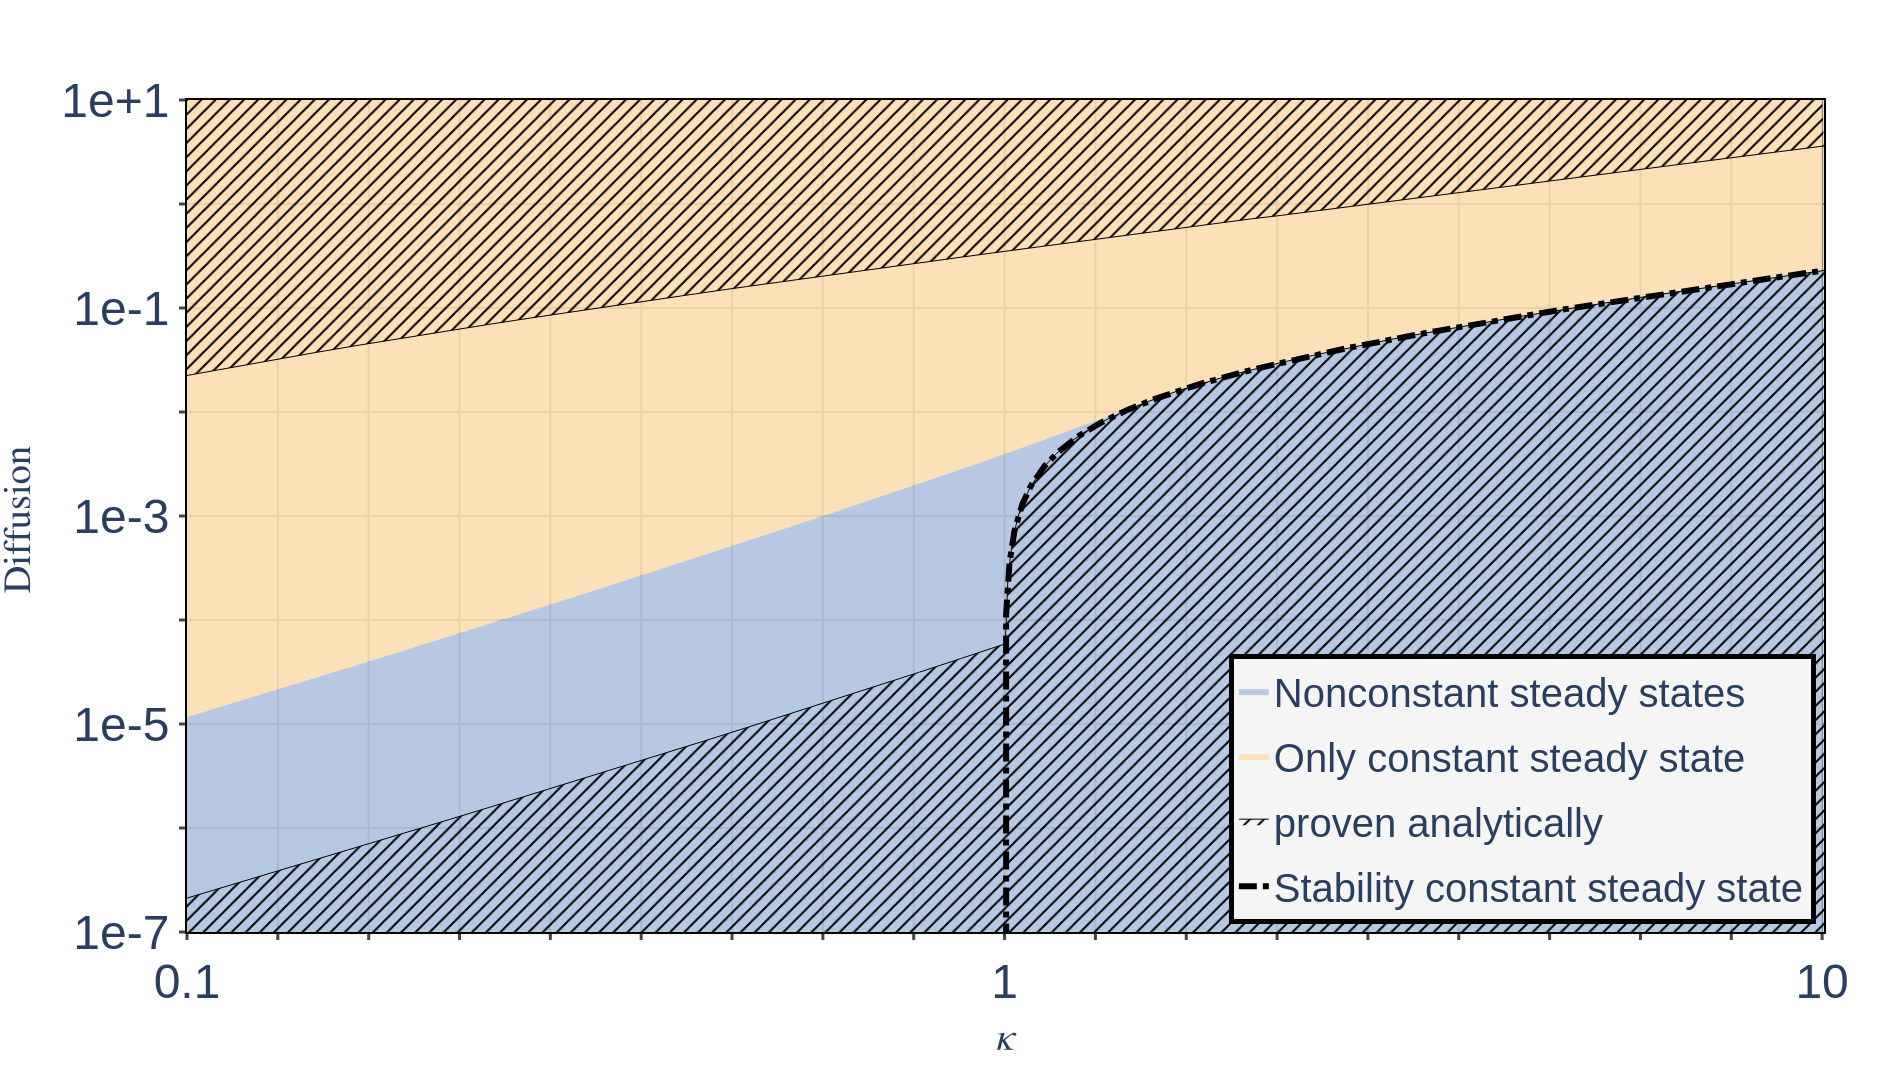
\includegraphics[
        width=\linewidth,
        height=5.35cm,
        keepaspectratio
      ]{figures/mechanochemistry/parameter_space.png}
    \end{column}

    \begin{column}{0.22\textwidth}
      \HydraPoint[HydraCyan]
        {Patterns}
        {Nonconstant steady states are found for sufficiently small diffusion}
      \vspace{-0.10cm}
      \HydraPoint[HydraGold]
        {Homogeneous state}
        {Large diffusion removes spatial variation}
      \vspace{-0.10cm}
      {\color{HydraMuted}\fontsize{6.9}{8.5}\selectfont
        Hatched regions are established analytically
      \par}
    \end{column}
  \end{columns}

\end{frame}


\begin{frame}{Linearization asks whether a stationary profile amplifies perturbations}

  \vspace{-0.10cm}

  {\color{HydraWhite}\fontsize{9.8}{12.4}\selectfont
  \begin{align*}
    u(x,t)&=U(x)+e^{\nu t}\varphi(x)
  \end{align*}
  }

  \vspace{-0.36cm}

  {\color{HydraMuted}\fontsize{7.6}{9.3}\selectfont
    Keeping only first-order terms gives the nonlocal eigenvalue problem
  \par}

  \vspace{-0.24cm}

  {\color{HydraWhite}\fontsize{8.7}{11}\selectfont
  \begin{align*}
    D\partial_{xx}\varphi
    +\left(
      \kappa\frac{e^U}{\int_0^1e^U}-1-\nu
    \right)\varphi
    &=
    \kappa
    \frac{e^U}{\left(\int_0^1e^U\right)^2}
    \int_0^1e^U\varphi
  \end{align*}
  }

  \vspace{-0.24cm}

  \begin{columns}[T,onlytextwidth]
    \begin{column}{0.48\textwidth}
      \HydraPoint[HydraCyan]
        {$\nu<0$}
        {The corresponding perturbation decays}
    \end{column}
    \begin{column}{0.48\textwidth}
      \HydraPoint[HydraGold]
        {$\nu>0$}
        {The corresponding perturbation grows}
    \end{column}
  \end{columns}

\end{frame}


\begin{frame}{A local problem helps locate the nonlocal eigenvalues}

  \vspace{-0.08cm}

  \begin{columns}[c,onlytextwidth]
    \begin{column}{0.48\textwidth}
      \centering
      {\color{HydraGold}\bfseries\fontsize{7.8}{9.4}\selectfont
        NONLOCAL PROBLEM\par}
      \vspace{-0.24cm}
      {\color{HydraWhite}\fontsize{8.7}{11}\selectfont
      \begin{align*}
        D\partial_{xx}\varphi
        +(A-\nu)\varphi
        &=MC(x)\int_0^1C(y)\varphi(y)\,dy
      \end{align*}
      }
      \par
      \vspace{-0.28cm}
      {\color{HydraMuted}\fontsize{7.2}{8.8}\selectfont
        Every value of $\varphi$ is coupled through the integral
      \par}
    \end{column}

    \begin{column}{0.48\textwidth}
      \centering
      {\color{HydraCyan}\bfseries\fontsize{7.8}{9.4}\selectfont
        LOCAL PROBLEM\par}
      \vspace{-0.24cm}
      {\color{HydraWhite}\fontsize{8.7}{11}\selectfont
      \begin{align*}
        D\partial_{xx}\psi
        +(A-\lambda)\psi
        &=0
      \end{align*}
      }
      \par
      \vspace{-0.28cm}
      {\color{HydraMuted}\fontsize{7.2}{8.8}\selectfont
        Classical oscillation theory orders the eigenfunctions by their zeros
      \par}
    \end{column}
  \end{columns}

  \vspace{0.36cm}

  \HydraTakeaway{
    Relevant nonlocal eigenvalues lie between eigenvalues of the associated local problem
  }

\end{frame}


\begin{frame}{Stable mechanochemical patterns are necessarily unimodal}

  \vspace{-0.16cm}

  \begin{columns}[c,onlytextwidth]
    \begin{column}{0.52\textwidth}
      \centering
      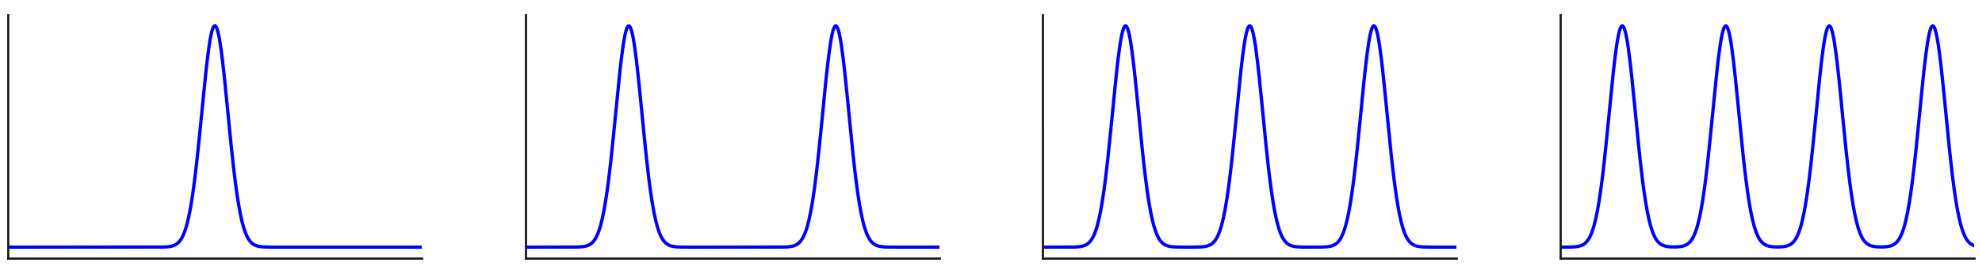
\includegraphics[
        width=\linewidth,
        height=4.65cm,
        keepaspectratio
      ]{figures/mechanochemistry/one_two_peaks.png}
    \end{column}

    \begin{column}{0.44\textwidth}
      {\color{HydraGold}\bfseries\fontsize{8.2}{9.8}\selectfont
        THEOREM\par}
      \vspace{0.16cm}
      \HydraPoint[HydraGreen]
        {Stable nonconstant solution}
        {The stable solution obtained by energy minimization has one peak}
      \vspace{-0.06cm}
      \HydraPoint[HydraRed]
        {Every multimodal solution}
        {All solutions with two or more peaks are linearly and nonlinearly unstable}
      \vspace{-0.06cm}
      {\color{HydraMuted}\fontsize{7.2}{8.8}\selectfont
        The global mechanical constraint strongly selects a single organizer
      \par}
    \end{column}
  \end{columns}

\end{frame}


\begin{frame}{Diffusion changes the width but not the number of stable peaks}

  \vspace{-0.14cm}

  \begin{columns}[c,onlytextwidth]
    \begin{column}{0.72\textwidth}
      \centering
      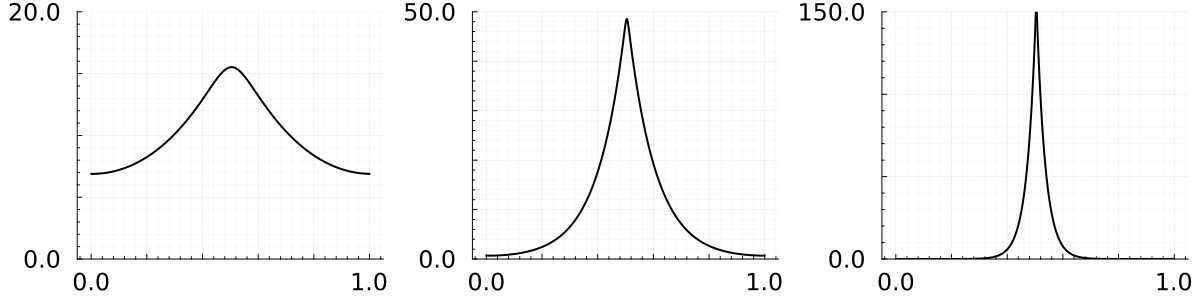
\includegraphics[
        width=\linewidth,
        height=5.15cm,
        keepaspectratio
      ]{figures/mechanochemistry/stationary_profiles.png}
    \end{column}

    \begin{column}{0.24\textwidth}
      \HydraPoint[HydraGold]
        {Smaller diffusion}
        {The stable peak becomes sharper and more localized}
      \vspace{-0.04cm}
      \HydraPoint[HydraCyan]
        {Larger diffusion}
        {The stable profile becomes broader}
      \vspace{-0.04cm}
      \HydraPoint[HydraGreen]
        {Robust selection}
        {The stable pattern retains a single dominant peak}
    \end{column}
  \end{columns}

\end{frame}


\HydraSubsection[
  \mbox{Stationary branches emerge when} \mbox{a homogeneous state changes stability} \mbox{and can generate tissue oscillations}
]{Bifurcations and oscillations}


\begin{frame}{A bifurcation marks a qualitative change in stationary states}

  \vspace{-0.16cm}

  \begin{columns}[c,onlytextwidth]
    \begin{column}{0.57\textwidth}
      \centering
      \begin{tikzpicture}[x=0.88cm,y=0.90cm]
        \draw[-{Latex[length=2.2mm]},HydraMuted,line width=0.75pt]
          (0.45,2.60) -- (7.75,2.60)
          node[anchor=north east,text=HydraMuted,font=\fontsize{7}{8.2}\selectfont] {control parameter $\kappa$};
        \draw[-{Latex[length=2.2mm]},HydraMuted,line width=0.75pt]
          (0.70,0.35) -- (0.70,5.35)
          node[left,text=HydraMuted,font=\fontsize{7}{8.2}\selectfont] {pattern amplitude};

        \draw[HydraCyan,line width=1.65pt]
          (0.75,2.60) -- (7.25,2.60);
        \draw[HydraGold,line width=1.75pt,domain=4.20:7.15,samples=80]
          plot (\x,{2.60+0.78*sqrt(\x-4.20)});
        \draw[HydraGold,line width=1.75pt,domain=4.20:7.15,samples=80]
          plot (\x,{2.60-0.78*sqrt(\x-4.20)});

        \draw[dashed,HydraLine,line width=0.8pt]
          (4.20,0.55) -- (4.20,4.95);
        \fill[HydraWhite] (4.20,2.60) circle[radius=0.085cm];

        \node[anchor=south,text=HydraWhite,
          font=\bfseries\fontsize{7.4}{8.9}\selectfont]
          at (4.20,5.02) {bifurcation point};
        \node[anchor=south west,text=HydraCyan,
          font=\fontsize{7.2}{8.7}\selectfont]
          at (1.20,2.72) {homogeneous state};
        \node[anchor=south west,text=HydraGold,
          font=\fontsize{7.2}{8.7}\selectfont]
          at (5.45,4.25) {patterned states};
      \end{tikzpicture}
    \end{column}

    \begin{column}{0.39\textwidth}
      \HydraPoint[HydraCyan]
        {Before the threshold}
        {Only the homogeneous stationary state is visible nearby}
      \vspace{0.02cm}
      \HydraPoint[HydraGold]
        {At the threshold}
        {A spatial mode becomes neutral and a patterned branch can emerge}
      \vspace{0.02cm}
      \HydraPoint[HydraGold]
        {After the threshold}
        {The number or stability of stationary states has changed}
    \end{column}
  \end{columns}

\end{frame}


\begin{frame}{The homogeneous state loses stability at discrete thresholds}

  \vspace{-0.22cm}

  {\color{HydraWhite}\fontsize{9.6}{12.1}\selectfont
  \begin{align*}
    \bar U&\equiv\kappa
    &
    \varphi_n(x)&=\cos(2\pi n x)
  \end{align*}
  }

  \vspace{-0.44cm}

  {\color{HydraMuted}\fontsize{7.6}{9.3}\selectfont
    Linearization assigns one growth rate to every spatial mode
  \par}

  \vspace{-0.26cm}

  {\color{HydraWhite}\fontsize{10.6}{13.4}\selectfont
  \begin{align*}
    \nu_n&=\kappa-1-4\pi^2n^2D
  \end{align*}
  }

  \vspace{-0.42cm}

  {\color{HydraGold}\bfseries\fontsize{11.2}{14.2}\selectfont
  \begin{align*}
    \boxed{\kappa_n=1+4\pi^2n^2D}
  \end{align*}
  }

  \vspace{-0.34cm}

  \begin{columns}[T,onlytextwidth]
    \begin{column}{0.31\textwidth}
      \HydraPoint[HydraGold]
        {$n=1$}
        {The first nonconstant mode has one maximum and one minimum}
    \end{column}
    \begin{column}{0.31\textwidth}
      \HydraPoint[HydraGold]
        {$n=2$}
        {The next mode produces a two-peak spatial structure}
    \end{column}
    \begin{column}{0.31\textwidth}
      \HydraPoint[HydraCyan]
        {Discrete thresholds}
        {Each mode changes stability at its own value of $\kappa$}
    \end{column}
  \end{columns}

\end{frame}


\begin{frame}{The first patterned branch can be subcritical or supercritical}

  \vspace{-0.12cm}

  {\color{HydraGold}\bfseries\fontsize{8.2}{9.8}\selectfont
    THEOREM\par}

  \vspace{0.20cm}

  {\color{HydraWhite}\fontsize{8.8}{11.1}\selectfont
    At $\kappa=\kappa_n$ a branch of nonconstant stationary solutions bifurcates from the homogeneous state $\bar U\equiv\kappa$
  \par}

  \vspace{0.24cm}

  \begin{columns}[T,onlytextwidth]
    \begin{column}{0.47\textwidth}
      \HydraPoint[HydraGold]
        {Subcritical branch}
        {$\kappa_n<3/2$ equivalently $D<(8\pi^2n^2)^{-1}$}
    \end{column}
    \begin{column}{0.47\textwidth}
      \HydraPoint[HydraCyan]
        {Supercritical branch}
        {$\kappa_n>3/2$ equivalently $D>(8\pi^2n^2)^{-1}$}
    \end{column}
  \end{columns}

  \vspace{0.32cm}

  {\color{HydraMuted}\fontsize{7.6}{9.3}\selectfont
    Near the bifurcation only the supercritical branch generated by the first mode can be stable
  \par}

  \vspace{0.16cm}

  \HydraTakeaway{
    The direction of the branch determines whether small patterned states appear before or after the linear threshold
  }

\end{frame}


\begin{frame}{Diffusion determines the type of each bifurcation}

  \vspace{-0.14cm}

  \begin{columns}[c,onlytextwidth]
    \begin{column}{0.73\textwidth}
      \centering
      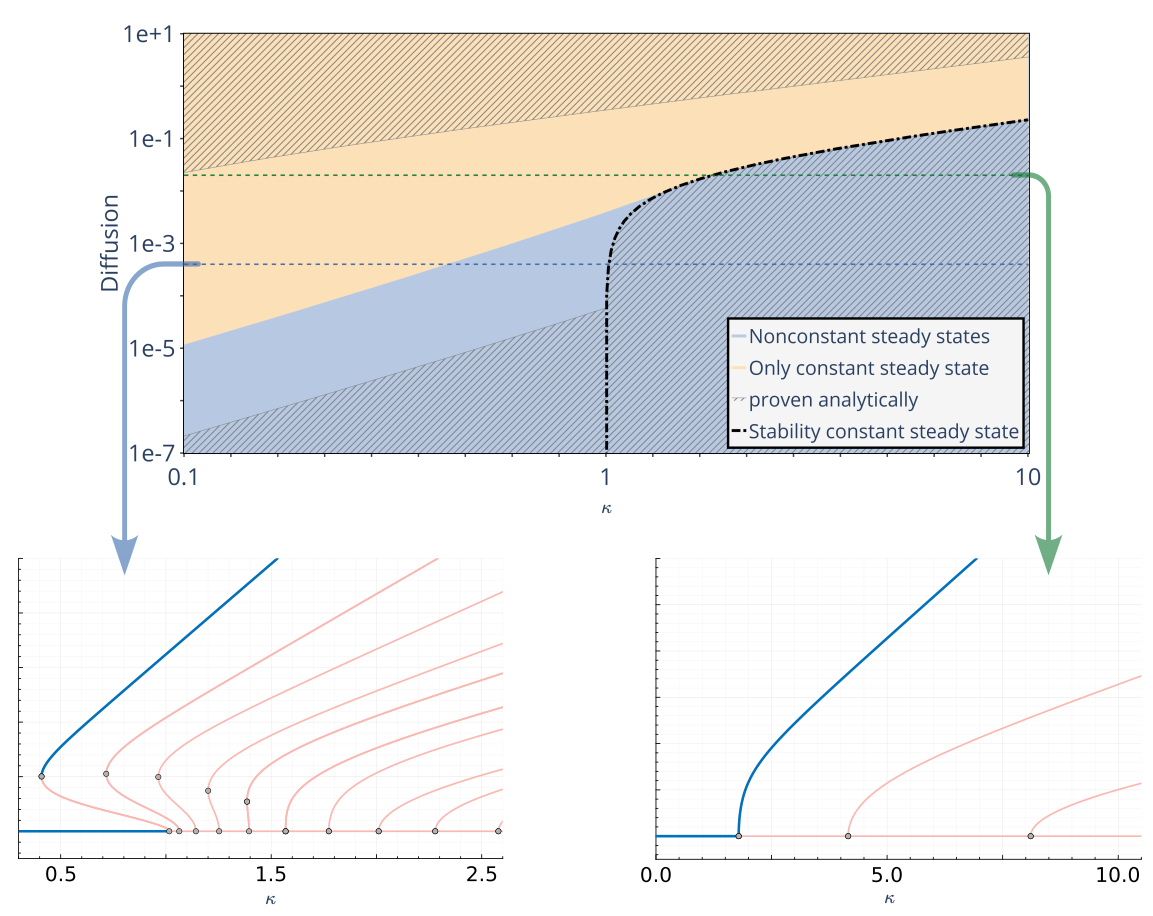
\includegraphics[
        width=\linewidth,
        height=5.25cm,
        keepaspectratio
      ]{figures/mechanochemistry/bifurcation_parameter_map.png}
    \end{column}

    \begin{column}{0.23\textwidth}
      \HydraPoint[HydraGold]
        {Small diffusion}
        {The branch can bend toward smaller values of $\kappa$}
      \vspace{0.04cm}
      \HydraPoint[HydraCyan]
        {Larger diffusion}
        {The branch can emerge toward larger values of $\kappa$}
      \vspace{0.04cm}
      {\color{HydraMuted}\fontsize{7.0}{8.6}\selectfont
        Each spatial mode has its own transition curve
      \par}
    \end{column}
  \end{columns}

\end{frame}


\begin{frame}{Tissue length turns the stationary picture into dynamics}

  \vspace{-0.18cm}

  {\color{HydraMuted}\fontsize{7.6}{9.3}\selectfont
    Let $\ell(t)$ denote the current circumference and $L$ its reference value
  \par}

  \vspace{-0.22cm}

  {\color{HydraWhite}\bfseries\fontsize{10.2}{12.9}\selectfont
  \begin{align*}
    \boxed{
      \partial_tu
      =
      D\partial_{xx}u-u
      +\kappa\bigl(\ell(t)-L\bigr)
      \frac{e^{u(x,t)}}{\int_0^1e^{u(y,t)}\,dy}
    }
  \end{align*}
  }

  \vspace{-0.34cm}

  \begin{columns}[T,onlytextwidth]
    \begin{column}{0.31\textwidth}
      \HydraPoint[HydraGold]
        {Morphogen rises}
        {The tissue softens and the mechanical equilibrium shifts}
    \end{column}
    \begin{column}{0.31\textwidth}
      \HydraPoint[HydraCyan]
        {The spheroid expands}
        {Increased strain strengthens morphogen production}
    \end{column}
    \begin{column}{0.31\textwidth}
      \HydraPoint[HydraGold]
        {Feedback relaxes}
        {Degradation and mechanical restoration can reverse the expansion}
    \end{column}
  \end{columns}

  \vspace{0.18cm}

  \HydraTakeaway{
    Coupling pattern formation to tissue size creates a route from static symmetry breaking to oscillations
  }

\end{frame}


\begin{frame}{Subcritical feedback permits abrupt switching}

  \vspace{-0.12cm}

  \begin{columns}[c,onlytextwidth]
    \begin{column}{0.62\textwidth}
      \centering
      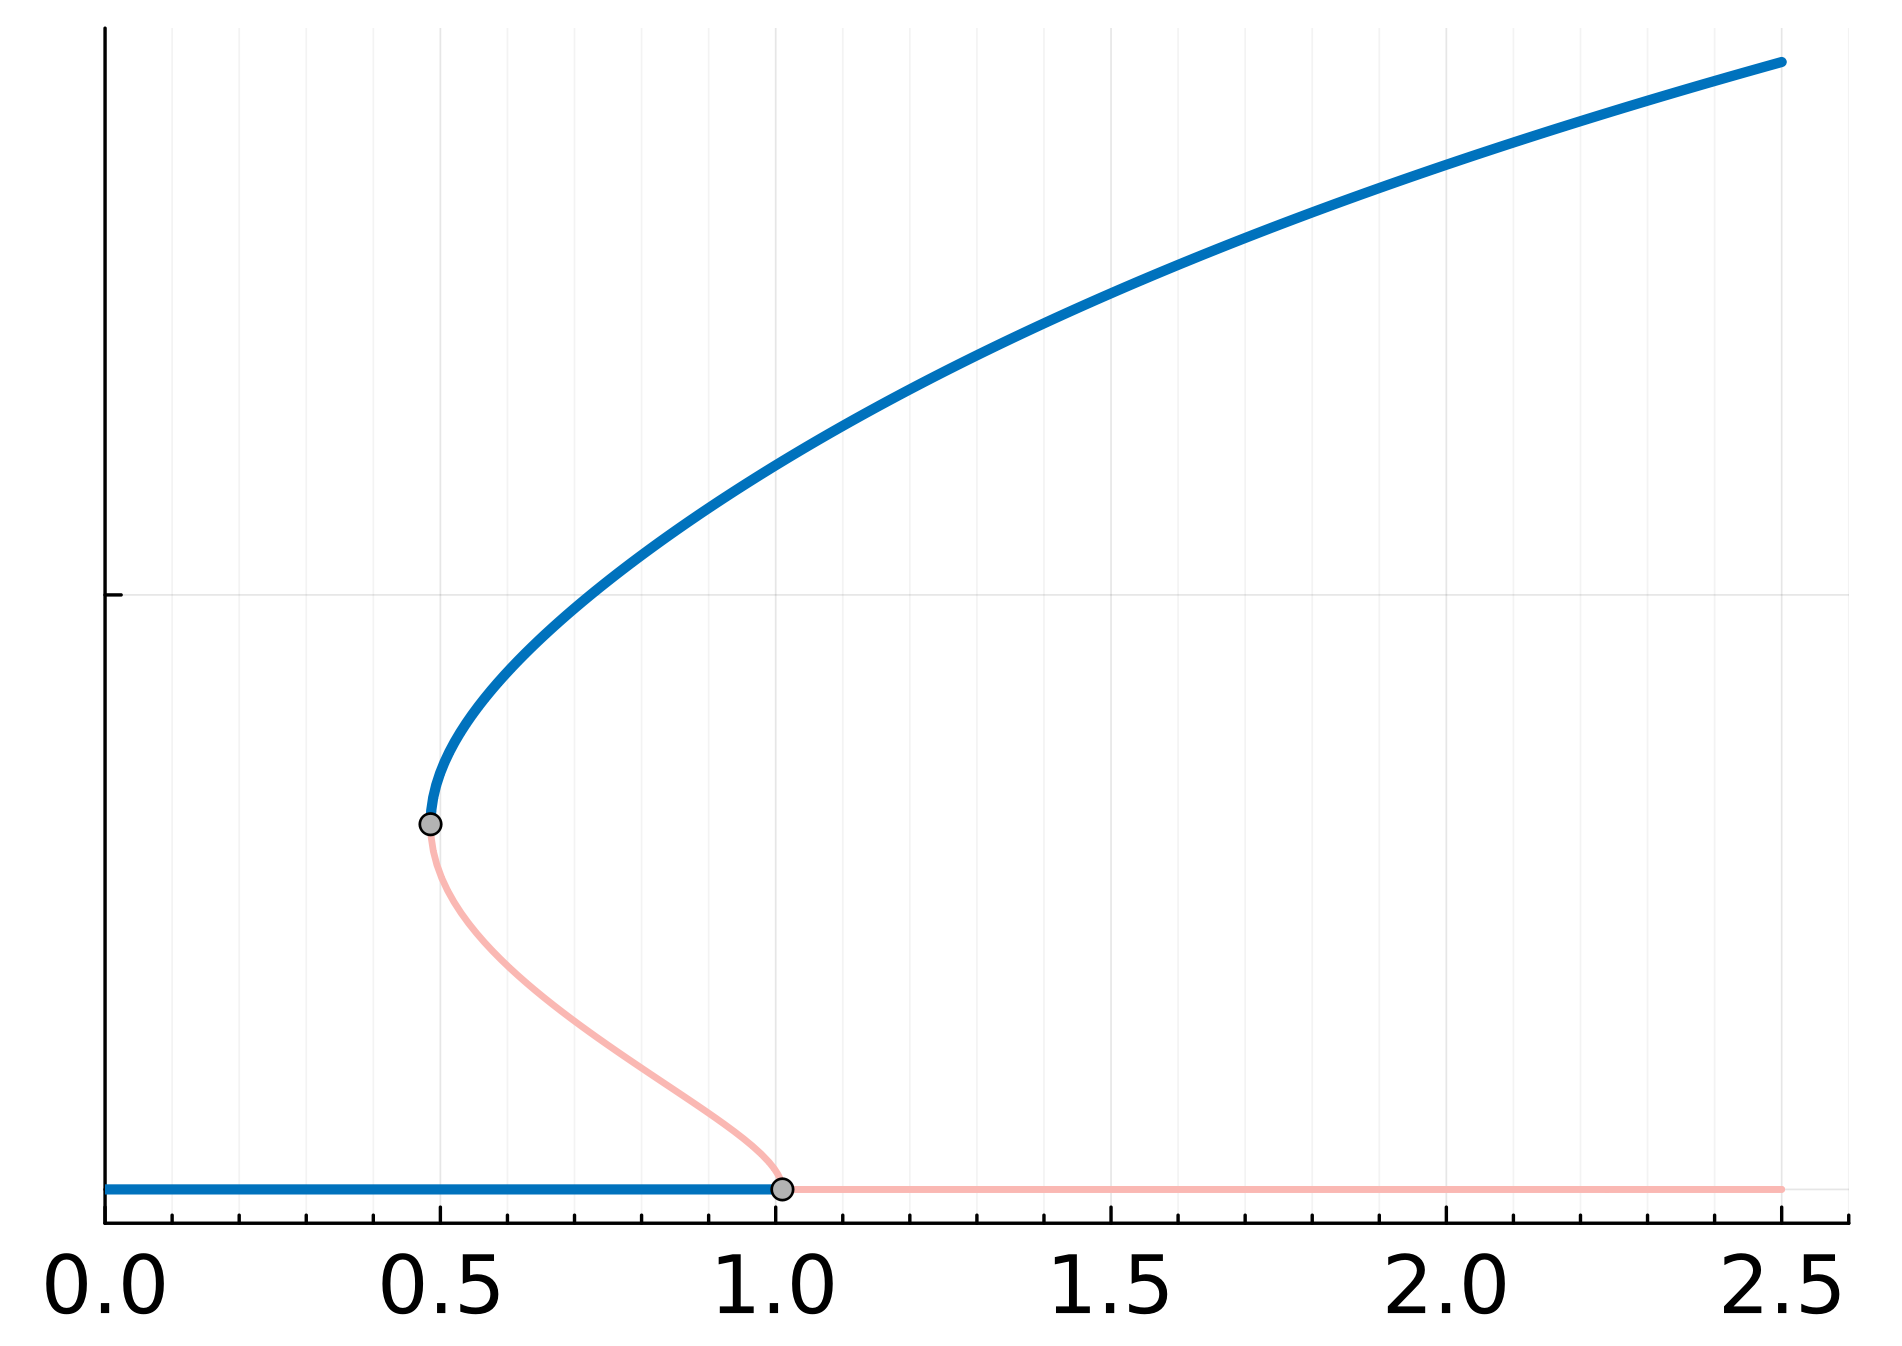
\includegraphics[
        width=\linewidth,
        height=5.05cm,
        keepaspectratio
      ]{figures/mechanochemistry/subcritical_bifurcation.png}
    \end{column}

    \begin{column}{0.34\textwidth}
      \HydraPoint[HydraGold]
        {Coexisting states}
        {A homogeneous and a patterned state may be available for the same parameter value}
      \vspace{0.04cm}
      \HydraPoint[HydraRed]
        {Sudden transition}
        {Crossing a fold can force the system to jump to a distant branch}
    \end{column}
  \end{columns}

\end{frame}


\begin{frame}{Supercritical feedback produces a gradual patterned response}

  \vspace{-0.12cm}

  \begin{columns}[c,onlytextwidth]
    \begin{column}{0.62\textwidth}
      \centering
      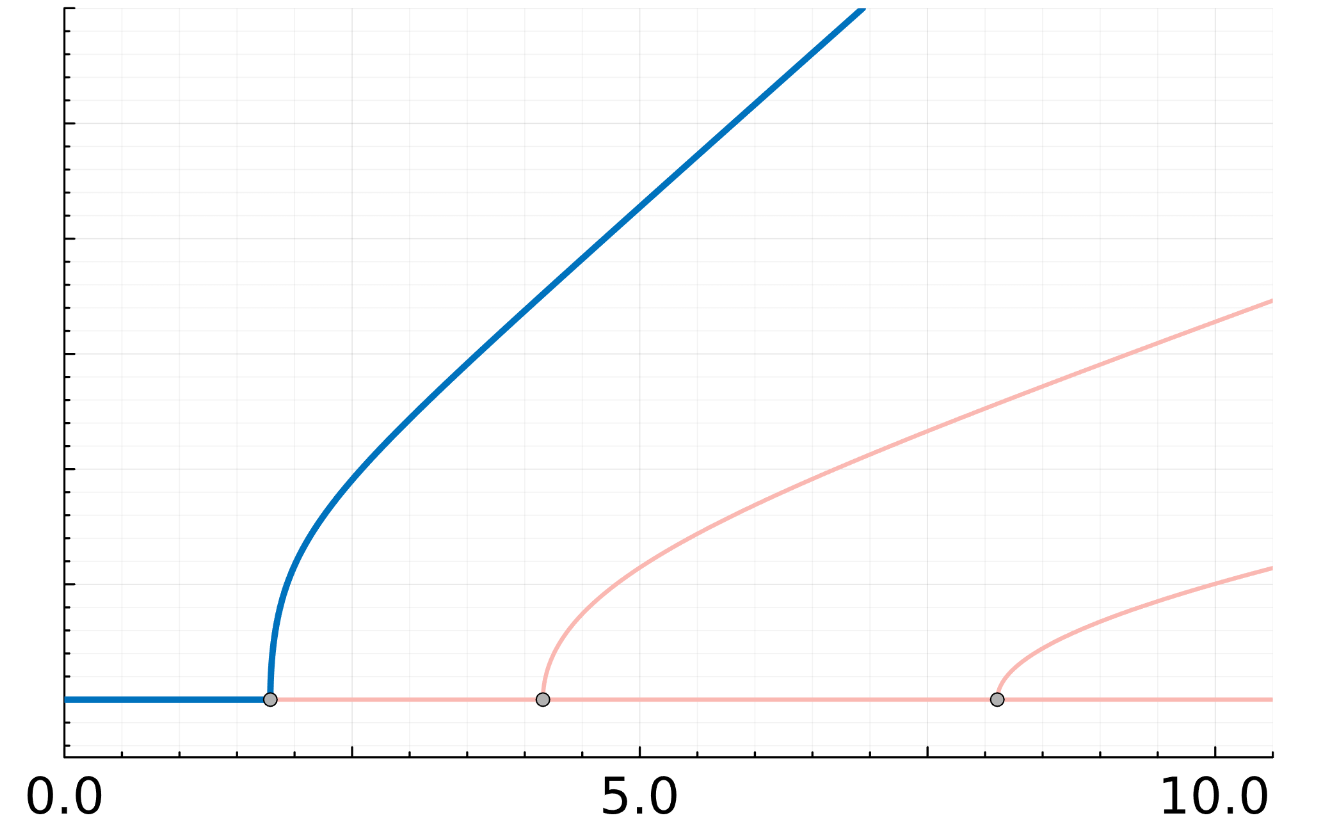
\includegraphics[
        width=\linewidth,
        height=5.05cm,
        keepaspectratio
      ]{figures/mechanochemistry/supercritical_bifurcation.png}
    \end{column}

    \begin{column}{0.34\textwidth}
      \HydraPoint[HydraCyan]
        {Continuous onset}
        {The patterned amplitude grows continuously from the homogeneous state}
      \vspace{0.04cm}
      \HydraPoint[HydraGold]
        {Smooth mechanical response}
        {Tissue deformation can track the changing stationary branch}
    \end{column}
  \end{columns}

\end{frame}


\begin{frame}{Mechanics can realize an activator--inhibitor mechanism without a chemical inhibitor}

  \vspace{-0.08cm}

  \begin{columns}[T,onlytextwidth]
    \begin{column}{0.31\textwidth}
      \HydraPoint[HydraGold]
        {Local positive feedback}
        {Stretch increases morphogen production and morphogen softens the tissue}
    \end{column}
    \begin{column}{0.31\textwidth}
      \HydraPoint[HydraCyan]
        {Global mechanical competition}
        {The fixed total length couples every point through one nonlocal constraint}
    \end{column}
    \begin{column}{0.31\textwidth}
      \HydraPoint[HydraGreen]
        {Single organizer}
        {Stable nonconstant stationary states contain one dominant peak}
    \end{column}
  \end{columns}

  \vspace{0.42cm}

  {\color{HydraWhite}\bfseries\fontsize{12.2}{15.2}\selectfont
  \begin{align*}
    \text{morphogen}
    \quad\Longrightarrow\quad
    \text{softening}
    \quad\Longrightarrow\quad
    \text{strain}
    \quad\Longrightarrow\quad
    \text{morphogen}
  \end{align*}
  }

  \vspace{-0.14cm}

  \HydraTakeaway{
    A single morphogen equation coupled to mechanics can implement local activation and long-range inhibition
  }

\end{frame}
